\clearpage
\section{V1 Development Gains and All-Object Changes}
The original development and new-scene plots are retained together with their exposure boundaries. ``Ours'' inside both plots denotes V1. The numerical tables and original predictions are unchanged.
\begin{center}
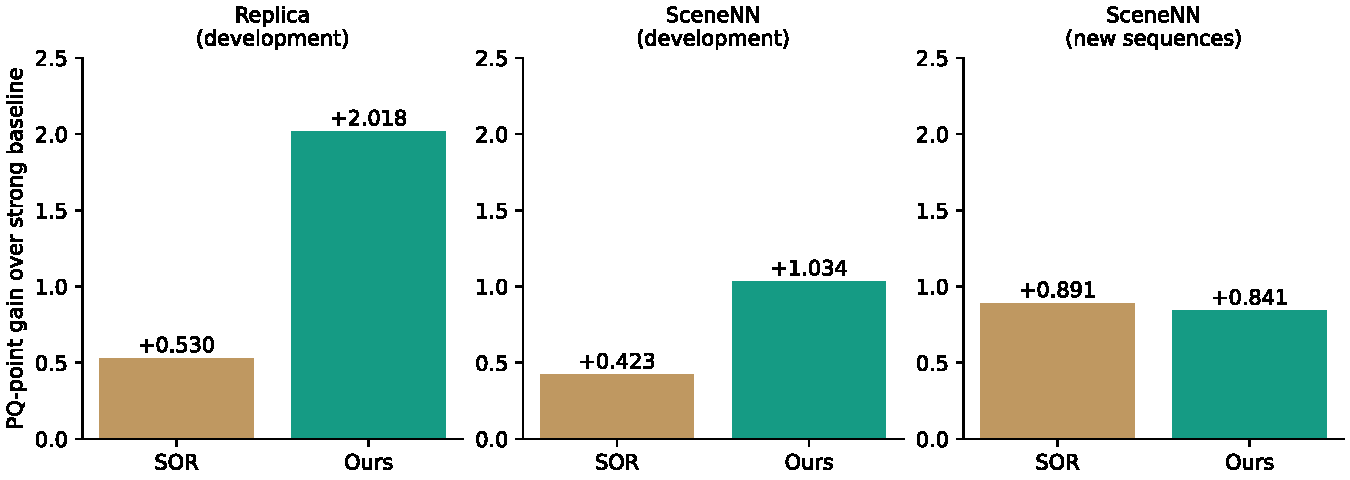
\includegraphics[width=\textwidth]{development_vs_unseen.pdf}
\captionof{figure}{PQ-point gains over the corresponding strong baseline, separated by dataset and development exposure. Replica office\_0/office\_1 and SceneNN 014/015 were exposed development scenes. Only the final group is the four new SceneNN sequences in the V1 main table. These gains do not describe current KITTI-360 authorization.}
\end{center}
\begin{center}
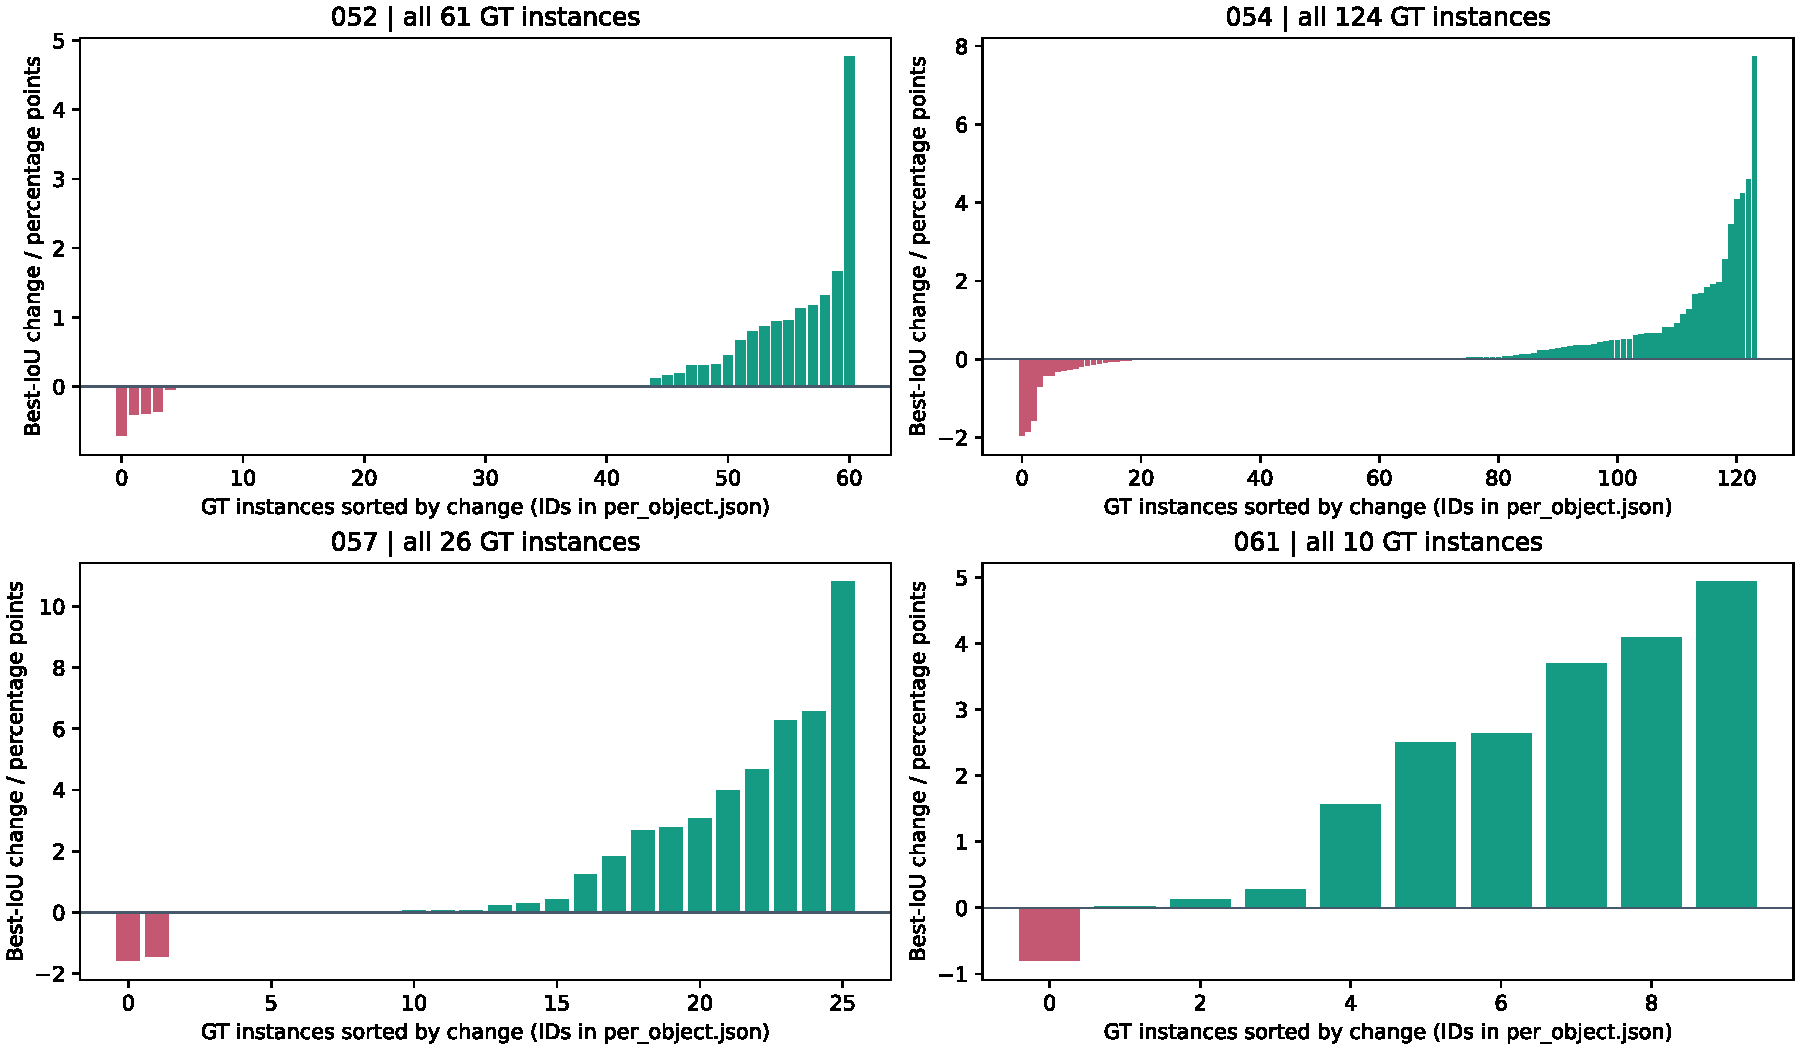
\includegraphics[width=\textwidth]{all_object_changes.pdf}
\captionof{figure}{Best-object IoU changes for all 221 GT instances in the four V1 SceneNN sequences. Objects are sorted by change within each scene; unchanged and regressed instances remain visible. There are 100 improvements, 27 declines, and 94 unchanged objects. Objects within a scene are not independent statistical trials.}
\end{center}

\clearpage
\section{V1 Evidence and Assignment Diagnostics}
These diagnostics explain why the V1 sequence-057 result trails SOR even though many individual geometries improve. They retain the original metric and the separately labeled locked-assignment diagnostic.
\begin{center}
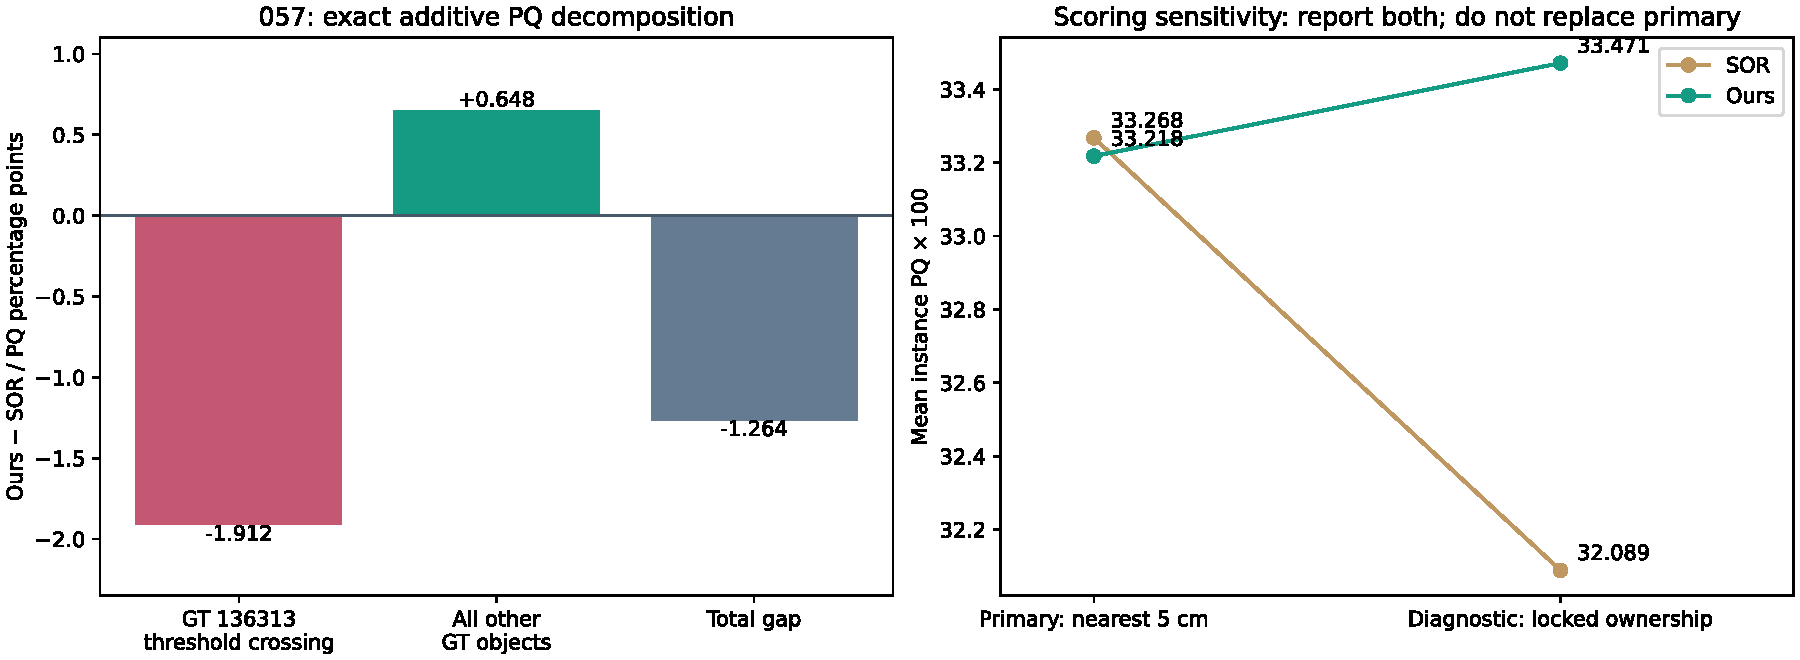
\includegraphics[width=\textwidth]{mechanism_decomposition.pdf}
\captionof{figure}{V1 sequence-057 primary-score deficit relative to SOR: one SOR-only match outweighs gains on the remaining objects. Locking baseline source ownership changes the mean ranking across four scenes. Locked assignment probes reference-label reassignment; it does not replace primary nearest-source evaluation. Embedded ``Ours'' means V1.}
\end{center}
\begin{center}
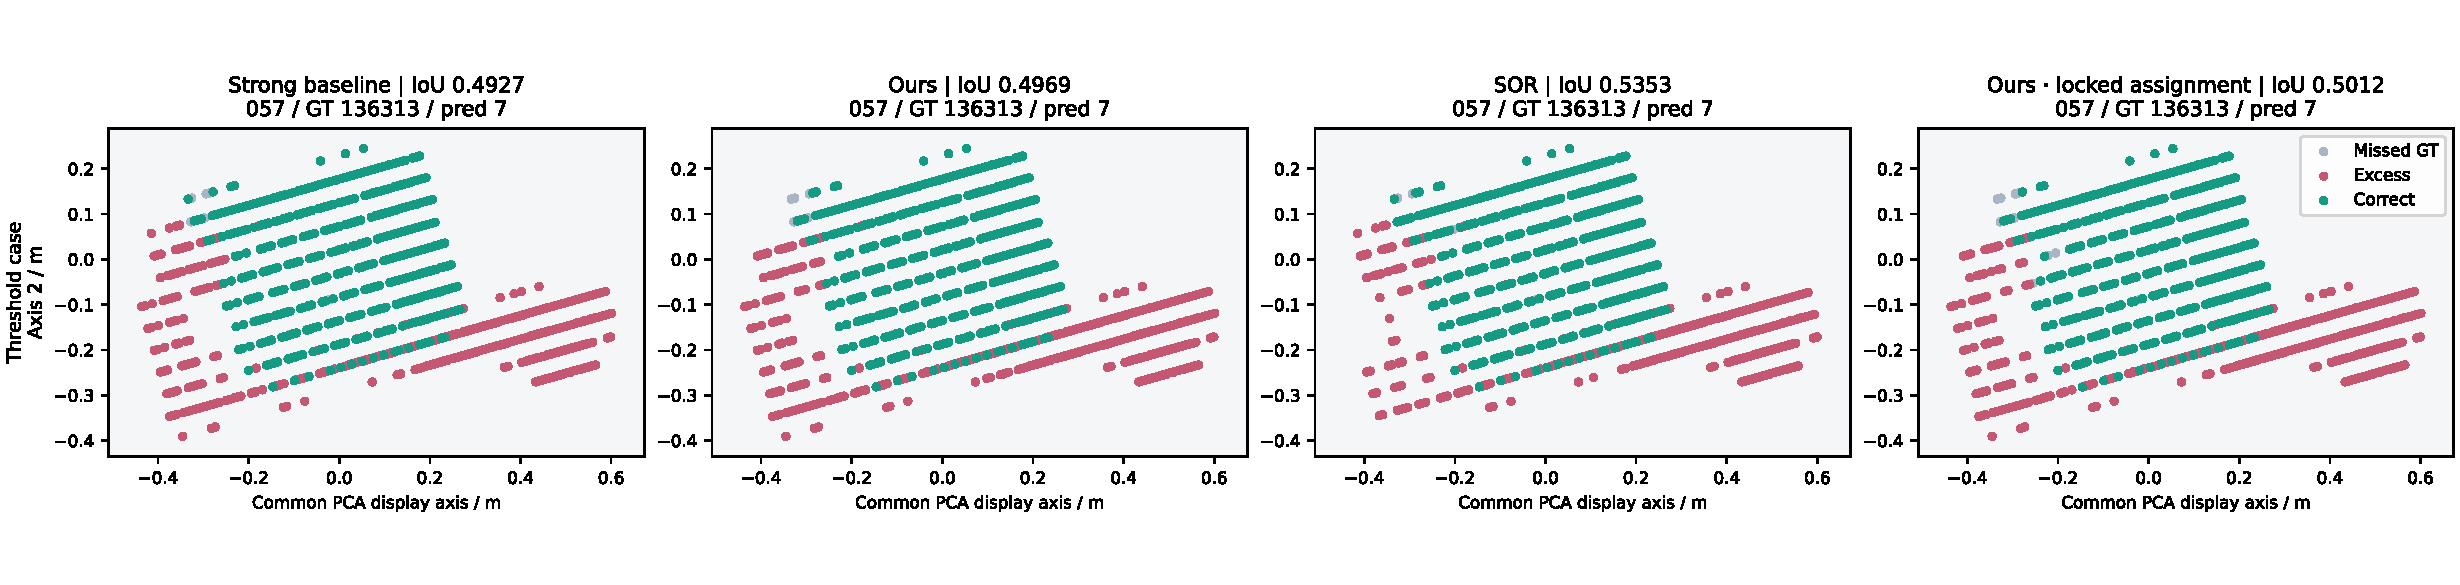
\includegraphics[width=\textwidth]{057_threshold_case.pdf}
\captionof{figure}{Threshold-sensitive GT object 136313 in a shared projection. Correct, excess, and missed reference support are green, red, and gray. The fourth panel locks baseline nearest-source ownership before deletion. All panels show the archived V1 study; ``Ours'' and ``Ours + locked assignment'' are not current-method results.}
\end{center}
The primary IoUs are 0.492718 (strong baseline), 0.496947 (V1), and 0.535340 (SOR). The locked V1 diagnostic is 0.501247. This case illustrates a threshold and ownership interaction, rather than evidence that deleting more points is necessarily better.
